% The parts of the Stage 2 report owned by Daniel Rodriguez (plan DR-15): the Indexing part of section 5, the
% storage and concurrency part of section 6, the Indexing part of section 7 and its consolidation. Section numbers
% follow the list of assignment section 7.1, where the cover is number 1. Same preamble as search_part.tex (DP-13).
%
% Build from docs/report/:  pdflatex indexing_part.tex && pdflatex indexing_part.tex
% The final report is report.tex. References to the sections of the others resolve only there.
\documentclass[11pt,a4paper]{article}

\usepackage[utf8]{inputenc}
\usepackage[T1]{fontenc}
\usepackage{lmodern}
\usepackage{microtype}
\usepackage[margin=2.4cm,headheight=14pt]{geometry}
\usepackage{graphicx}
\usepackage{booktabs}
\usepackage{tabularx}
\usepackage{array}
\usepackage{enumitem}
\usepackage{float}
\usepackage{xcolor}
\usepackage{listings}
\usepackage{fancyhdr}
\usepackage{titlesec}
\usepackage{tikz}
\usetikzlibrary{arrows.meta,positioning,fit,backgrounds,calc,shadows}
\usepackage[hidelinks]{hyperref}

\definecolor{accent}{HTML}{2a78d6}
\definecolor{ink}{HTML}{0b0b0b}
\definecolor{muted}{HTML}{52514e}
\definecolor{codebg}{HTML}{f6f6f4}
\definecolor{rule}{HTML}{d8d7d2}
\definecolor{pendingink}{HTML}{b3261e}

\hypersetup{colorlinks=true,linkcolor=accent,urlcolor=accent,citecolor=accent}

\titleformat{\section}{\Large\bfseries\color{ink}}{\thesection.}{0.6em}{}
\titleformat{\subsection}{\large\bfseries\color{ink}}{\thesubsection}{0.6em}{}
\titlespacing*{\section}{0pt}{1.6em}{0.7em}
\titlespacing*{\subsection}{0pt}{1.2em}{0.5em}

\pagestyle{fancy}
\fancyhf{}
\fancyhead[L]{\small\color{muted}Stage 2 $\cdot$ Service-oriented architecture}
\fancyhead[R]{\small\color{muted}Big Data $\cdot$ ULPGC}
\fancyfoot[C]{\small\thepage}
\renewcommand{\headrulewidth}{0.4pt}

\setlist{itemsep=2pt,topsep=4pt}
\setlength{\parskip}{0.45em}
\setlength{\parindent}{0pt}
\setlength{\emergencystretch}{3em}
\renewcommand{\arraystretch}{1.25}

\lstset{language={}, basicstyle=\ttfamily\footnotesize, backgroundcolor=\color{codebg}, frame=single,
  rulecolor=\color{rule}, framesep=4pt, xleftmargin=6pt, xrightmargin=6pt, breaklines=true,
  columns=fullflexible, keepspaces=true, showstringspaces=false, aboveskip=8pt, belowskip=8pt}

\newcolumntype{L}[1]{>{\raggedright\arraybackslash}p{#1}}
\newcommand{\code}[1]{\texttt{#1}}
\newcommand{\pending}[1]{\par\medskip{\color{pendingink}\textbf{[PENDING]} #1}\par\medskip}


\begin{document}

\tableofcontents
\clearpage

\setcounter{section}{4}
\section{Microservice implementation: Indexing}
\label{sec:indexing}

Indexing turns the complete books of the datalake into the inverted index and the metadata in MongoDB, and decides
when a new version of the index becomes visible to Search. It is written in Java 17 with Javalin and Gson. Its HTTP
API, \code{api/indexing-openapi.yaml}, has five endpoints: \code{POST /index/update/\{book\_id\}} indexes one book,
\code{POST /index/publish} and \code{POST /index/rebuild} publish and rebuild the index, and \code{GET /index/status}
and \code{GET /status} report its state. Its MongoDB side is specified in \code{index-publication.md} and its
Hazelcast side in \code{coordination.md}, both in \code{api/contracts/}. Its main classes are:

\begin{table}[H]
\centering\small
\begin{tabularx}{\linewidth}{@{}L{5.3cm}>{\raggedright\arraybackslash}X@{}}
\toprule
\textbf{Class} & \textbf{Responsibility} \\
\midrule
\code{IndexingApi} & Validates the requests and turns results and exceptions into the HTTP answers of the contract \\
\code{IndexingService} & Reads, parses and tokenizes books, and writes them: one book (\code{update}) or a batch
  (\code{indexBatch}) \\
\code{IndexingWriter} & The consumer of \code{index-queue}: holds \code{index-writer}, claims batches, completes or
  fails each book \\
\code{LeaseRenewer} & Renews the leases of the batch being written \\
\code{Publisher} & Publishes a new version of the index with a conditional switch of \code{CURRENT} \\
\code{HazelcastPublicationNotifier} & After a publication, announces \code{IndexPublished} and marks the books
  \code{PUBLISHED}, in a thread of its own \\
\code{Rebuilder} & \code{POST /index/rebuild}: rebuilds the whole index into a new collection and switches to it \\
\code{MongoPublicationRepository} & The publication collections: \code{index\_meta}, \code{index\_books},
  \code{index\_publications}, \code{index\_log} \\
\bottomrule
\end{tabularx}
\caption{Structure of the Indexing Service. The datalake, the tokenizer, the metadata parser and the MongoDB stores of
the index and the metadata are in \code{common}, shared with the other services.}
\end{table}

\textbf{One book, one batch.} Both ways in index the same way, in two steps. \emph{Prepare} reads the header and the
body of each book from the datalake, parses the metadata (title, author, language, year) and tokenizes the body with the
tokenizer of Stage~1, the same one Search uses for queries: ASCII letters in lower case and digits, tokens of at least
2 characters, without stopwords. It runs in parallel on a pool of
\code{INDEXING\_THREADS} (4). \emph{Write} runs in one thread and in this order: the metadata of every book of the batch
with one bulk write into \code{books}, the posting lists with one bulk write into the inverted index, and \emph{last}
one entry per book in \code{index\_log}. The inverted index sends one \code{\$addToSet} upsert per \emph{distinct} term
of the batch, so a common word is written once per batch, not once per book. A book that cannot be prepared is left
out and reported, and never stops the others. A write that fails fails the whole batch.

\textbf{Why \code{index\_log} goes last.} It is the evidence that a book is complete in the index: the publication
takes its books from it, the book becomes \code{INDEXED} in Hazelcast only after it, and the recovery of the Control
(Section~\ref{sec:recovery}) reads it. A process that dies in the middle of a batch leaves no entry, so the book is
indexed again and never published half written.

\subsection{Readiness, task ownership and retries}

\textbf{Readiness.} Indexing reads a book only if its \code{\_READY} marker is in the datalake
(Section~\ref{sec:readiness}). Otherwise \code{POST /index/update} answers 404 and the queue writer fails the book with
\code{NOT\_READY}, which puts it back in the queue.

\textbf{Task ownership.} One thread per replica runs \code{IndexingWriter}. It first takes the Hazelcast lock
\code{index-writer}: only its holder consumes \code{index-queue}, and another replica waits as a standby and takes over
when the holder stops or dies. The holder claims a book, waiting for one, and then the books already waiting, without
waiting, up to \code{INDEX\_WRITE\_BATCH} (100). With few books a batch has one book and nothing waits for more; with a
backlog the batches fill up by themselves. After the write, it completes each indexed book (\code{INDEXED}). Each
claim has a lease of \code{LEASE\_SECONDS} (120~s). A batch on a large index can take longer than that (about 33~s per
batch at 10,000 books, Section~\ref{sec:benchmarks-indexing}), so \code{LeaseRenewer} renews the leases of the batch
every third of the lease while it is written. Without it, the Control would requeue books that are still being written.

\textbf{Retries.} Each failure goes back to Hazelcast with a code of the coordination contract:

\begin{table}[H]
\centering\small
\begin{tabularx}{\linewidth}{@{}L{4.6cm}L{4cm}X@{}}
\toprule
\textbf{Failure} & \textbf{Code} & \textbf{What happens} \\
\midrule
Book not complete in the datalake & \code{NOT\_READY} & Requeued, one attempt more \\
Book without indexable terms & \code{EMPTY\_BOOK} & \code{FAILED} at once; nothing is written \\
MongoDB does not answer & \code{STORAGE\_UNAVAILABLE} & The whole batch is requeued \emph{without} counting an attempt,
  and the writer waits 1, 2, 4\ldots{} up to 30~s before its next claim \\
Anything else & \code{INTERNAL\_ERROR} & Requeued, one attempt more \\
\bottomrule
\end{tabularx}
\caption{Failures of the queue writer.}
\end{table}

If completing or failing a book finds that its task changed, the writer had lost it (the Control requeued it after its
lease expired), and the result is dropped. When the client loses the cluster, the writer stops claiming at once, and
takes the lock again before writing anything when the cluster is back. In real failover runs, a standby replica
took over 2.8~s after a \code{SIGTERM} of the holder and 4.0~s after a \code{kill -9}, and the 17 books the dead holder had
claimed came back through their leases.

\subsection{Idempotency}

Indexing a book twice leaves the index exactly as indexing it once, so every retry is safe:
\begin{itemize}
  \item the posting lists use \code{\$addToSet}, so an id is never added twice, and the unique index on \code{term} keeps
        one document per term;
  \item \code{books} and \code{index\_log} are upserts by \code{\_id};
  \item two replicas, or two threads, writing the same new term at once meet on the unique index. MongoDB retries such
        an upsert by itself because its filter is an equality on the unique key, so neither fails.
\end{itemize}
A test with two \code{IndexingService} of 4 threads each, indexing the same books at once against a real MongoDB,
checks that the index ends as after a single run. \code{docs/robustness.md} lists each failure, what must happen and
the test that proves it, and the mutants those tests catch.

\subsection{Publication of completed index updates}

Search must never show a book half written, and must see all the books of a version at once. A version is a document
\code{CURRENT} in \code{index\_meta}, and a book is visible when \code{index\_books} gives it a version $\le$
\code{CURRENT}. \code{Publisher} publishes on top of \code{CURRENT} = V in four steps:
\begin{enumerate}
  \item the books to publish are those of \code{index\_log} that are not in \code{index\_books}: complete by
        construction;
  \item it records them in \code{index\_books} with version V+1, with \code{\$setOnInsert}: a book keeps forever the
        first version in which it became visible. Search still shows V;
  \item it switches \code{CURRENT} to V+1 \emph{only if it is still V}, a conditional update. This is the instant the
        books become visible, all at once;
  \item it writes the entry of V+1 in \code{index\_publications}, the history.
\end{enumerate}
A process that dies between steps 2 and 3 leaves books above \code{CURRENT}, invisible, and the next publication
completes them. If the conditional switch fails, another replica published first, and the publication is repeated on
top of the new \code{CURRENT}, up to 3 times. The Control decides \emph{when} to publish
(Section~\ref{sec:ingestion-control}); Indexing does it.

After answering, the publication is announced from a thread of its own: the \code{IndexPublished} event on
\code{index-events}, one per version and in order while connected, and the transition of the published books from
\code{INDEXED} to \code{PUBLISHED} in Hazelcast. A slow Hazelcast therefore never holds the publication nor its HTTP
request. Without the cluster the last version is kept and announced on reconnection; a lost event does no harm,
because Search also checks \code{CURRENT} every 5~s.

\subsection{Full rebuild of the index}

\code{POST /index/rebuild} indexes every complete book of the datalake again into a \emph{new} collection,
\code{inverted\_index\_rNN}, while Search keeps reading the current one. It is needed when the tokenizer changes, for
instance. Any replica can start it:
\begin{enumerate}
  \item it puts a marker in Hazelcast (\code{putIfAbsent} with a TTL of 30~s), so only one rebuild runs. While the
        marker exists no writer claims from the queue, and update and publish answer 409 in every replica. A thread of
        the rebuild renews the TTL every 10~s, also in the middle of a batch; if the replica dies, the marker expires
        and indexing goes on;
  \item it takes \code{index-writer}, which the queue writer releases at the end of its batch, and indexes every book
        into \code{rNN} in batches;
  \item a safety pass indexes into \code{rNN} every book published meanwhile in the old collection (a replica without
        Hazelcast does not see the marker);
  \item it switches with one more publication, V+1 on \code{rNN} with every book: Search sees the new collection, and
        every book, at once;
  \item the old collection is dropped after \code{INDEX\_REBUILD\_DROP\_SECONDS} (60~s), well above the 5~s in which a
        Search replica still serves its old snapshot.
\end{enumerate}
If anything fails before the switch, \code{rNN} is dropped and \code{CURRENT} is untouched.

\textbf{Availability.} \code{GET /status} never touches MongoDB, so it answers from the first second. The connection to
Hazelcast is made in the background after the HTTP server starts; until then, and whenever the cluster is lost,
\code{POST /index/update} and \code{POST /index/publish} keep working, because indexing a book does not need the
cluster. If MongoDB does not answer, they answer 503 \code{STORAGE\_UNAVAILABLE}, and retrying is safe.


\setcounter{section}{5}
\section{Design decisions: storage and concurrency}
\label{sec:decisions-storage}

\subsection{Storage selection}

Stage~1 compared several structures for each store and chose, for 200 books, a datalake with one folder per book and a
monolithic JSON inverted index. Stage~2 must index tens of thousands of books with several processes sharing the data,
so the group moved to structures that Stage~1 had already implemented and tested:

\begin{table}[H]
\centering\small
\begin{tabularx}{\linewidth}{@{}L{2.2cm}L{3.3cm}X@{}}
\toprule
\textbf{Store} & \textbf{Choice} & \textbf{Why} \\
\midrule
Datalake & \emph{range}: one folder per 1,000 ids, such as \code{01000-01999/} &
  With one folder per book the root holds one entry per book, hundreds of thousands. With \emph{range} each folder has
  at most about 3,000 files (header, body and \code{\_READY} of each book), and the folder of a book is computed from
  its id, never searched. Files are the cheapest way to keep raw text, and the only store on disk besides MongoDB. \\
Inverted index & MongoDB: one document \code{\{term, postings\}} per term, unique index on \code{term} &
  The monolithic JSON is held whole in memory and rewritten whole at each flush; Stage~1 itself noted that it had to
  change beyond about 2,000 books. In MongoDB a flush sends only the terms that changed, a query reads only the
  documents of its terms, and many processes can read and write it at once. \\
Metadata & MongoDB: collection \code{books}, one document per book &
  By volume SQLite was enough (about 30~MB for 100,000 books). The reason is Stage~3: a SQLite file cannot be shared
  between machines, and MongoDB was already deployed. Search reads the metadata by \code{\_id} and filters in memory. \\
Publication & MongoDB: four collections &
  \code{index\_meta}, \code{index\_books}, \code{index\_publications} and \code{index\_log}. The version of the index must change for Search in one atomic step, and a conditional update of one document
  (\code{CURRENT}) gives it without any lock (Section~\ref{sec:indexing}). \\
\bottomrule
\end{tabularx}
\caption{Storage of each kind of data. The datalake is the only persistent truth on disk; everything else is in one
MongoDB database.}
\label{tab:storage}
\end{table}

\textbf{What the measures say about this choice} (Section~\ref{sec:benchmarks-indexing}). With 30,000 books the index has
651,565 terms and 94.7 million ids, and takes 1.11~GB on disk. Its longest posting list, the word \emph{said}, holds
29,898 ids in 318~KB: far from the 16~MB limit of a MongoDB document, and reading it takes 2.8~ms. One document per
term is therefore enough for queries at this scale. The cost is on the write side. \code{\$addToSet} compares each new
id with the whole list to keep it free of duplicates, so adding 100 ids costs 6~ms on a list of 1,000 ids and 233~ms on
one of 100,000. Since the frequent terms hold almost one id per book, every batch pays for the size of the index, and
the indexing rate falls from about 17 to 1 book per second between an empty index and 30,000 books.

\textbf{What would fix it, and why it was not done.} \code{\$push} is 14 to 20 times faster on long lists, but it accepts
duplicates, and idempotency is what makes every retry of the pipeline safe (Section~\ref{sec:indexing}). Avoiding
duplicates without \code{\$addToSet} would need another mechanism, such as writing a batch only once per book with a
check in \code{index\_log}. The other option is to split each posting list into buckets of bounded size, which keeps
\code{\$addToSet} cheap but changes the contract of the index and the reads of Search. Both are proposed for Stage~3, not
measured.

\subsection{Concurrency model of Indexing}

One Indexing process runs these threads:

\begin{table}[H]
\centering\small
\begin{tabularx}{\linewidth}{@{}L{3.6cm}L{2.2cm}X@{}}
\toprule
\textbf{Threads} & \textbf{How many} & \textbf{What they do} \\
\midrule
Jetty pool & up to \code{INDEXING\_HTTP\_THREADS} (250) & One per HTTP request \\
Parsers & \code{INDEXING\_THREADS} (4) & Read, parse and tokenize the books of a batch, in parallel \\
Queue writer & 1 & Holds \code{index-writer}, claims, writes, completes \\
Lease renewer & 1 & Renews the leases of the batch being written \\
Notifier & 1 & Announces each publication and marks its books \code{PUBLISHED} \\
Rebuild & 1, and 1 for its marker & Only while a rebuild runs \\
\bottomrule
\end{tabularx}
\caption{Threads of one Indexing process. The Hazelcast client and the MongoDB driver add their own.}
\end{table}

\textbf{Many parsers, one writer.} Preparing a book is pure CPU and independent of the others, so it runs in parallel.
Writing is not: the pending changes of the inverted index are one map per process, and the order of the writes
(metadata, posting lists, \code{index\_log}) is what makes a book complete. So writes go one at a time, whether they come
from the queue writer or from \code{POST /index/update}. Between replicas, the \code{index-writer} lock leaves a single
writer in the whole system; more replicas are standbys for failover, not more throughput. A second writer would update
the same documents as the first, because the frequent terms are in almost every book: the two would contend on the same
posting lists in MongoDB and add no capacity where it is missing.

\textbf{Protection of the shared state.}

\begin{table}[H]
\centering\small
\begin{tabularx}{\linewidth}{@{}L{3.6cm}L{3.8cm}X@{}}
\toprule
\textbf{Shared state} & \textbf{Shared by} & \textbf{Protection} \\
\midrule
Pending posting lists & Threads of one process & A lock around add and flush \\
Writing the index & Replicas of Indexing & Hazelcast lock \code{index-writer}, held by one thread \\
Leases of the claimed books & Writer and Control & Conditional replace of the task in \code{book-state} \\
\code{CURRENT} & Replicas that publish & Conditional update: only from V to V+1 \\
Version of a published book & Publications & \code{\$setOnInsert}: it never changes \\
Posting lists and metadata & Replicas, retries & Idempotent writes: \code{\$addToSet}, upserts by \code{\_id} \\
Rebuild marker & Replicas & \code{putIfAbsent} with a TTL and a token; renewed and removed only by its owner \\
\bottomrule
\end{tabularx}
\caption{How Indexing protects each piece of shared state.}
\end{table}

\subsection{Where threads and replicas help, and where they contend}

\begin{itemize}
  \item \textbf{More parser threads help the CPU part only.} Alone, preparing a batch goes from 233 to 487 books per
        second between 1 and 8 threads, and stops improving at 4. Inside the deployment the whole path into MongoDB
        stays at 15 books per second whatever the threads: CPU is not what limits indexing.
  \item \textbf{More Indexing replicas do not add throughput} by design: they are standbys. What they add is
        failover, measured at 2.8 to 4.0~s.
  \item \textbf{MongoDB is the shared resource.} Indexing writes the index that Search reads. With the pipeline
        running, Indexing processed 2.42 books per second alone and 0.91 while Search was under load, and with 128
        clients the p95 of Search rose from 109 to 160~ms. On one host they also share its CPUs.
  \item \textbf{What would help}, for Stage~3: a cheaper write than \code{\$addToSet} on long lists, a larger MongoDB
        cache (the index exceeds its 0.25~GB from about 10,000 books), and MongoDB on a machine of its own, away from
        the other services.
\end{itemize}


\setcounter{section}{6}
\section{Benchmarks and results: Indexing}
\label{sec:benchmarks-indexing}

Indexing was measured at two levels: its CPU work alone with JMH on the host, and the whole path from
\code{index-queue} into MongoDB with the real services in Docker Compose. The scripts, the instructions to repeat every
measure and the raw results are in \code{benchmarks/indexing/}; the figures come from \code{benchmarks/plot.py}.

\subsection{Microbenchmarks with JMH}

The benchmarks live in the test code of \code{indexing-service}, package \code{...indexing.benchmark}, and run from the
benchmarks jar on the reference machine (Section~\ref{sec:consolidation}): 2 forks with a 4~GB heap, 5 warm-up and 10
measured iterations of 1~s each (20 samples), average time per operation with its 99.9~\% error. The books are three synthetic bodies of the dataset (short, median
and long), read from the page cache, so the benchmarks measure CPU, not disk.

\begin{table}[H]
\centering\small
\begin{tabularx}{\linewidth}{@{}Xrl@{}}
\toprule
\textbf{Benchmark} & \textbf{Time ($\mu$s)} & \textbf{Derived} \\
\midrule
Tokenize a short body (6.8~KB) & 114 $\pm$ 8 & 60 MB/s \\
Tokenize the median body (49.6~KB) & 844 $\pm$ 66 & 59 MB/s \\
Tokenize a long body (281.5~KB) & 5,137 $\pm$ 310 & 55 MB/s \\
Parse a header & 21.2 $\pm$ 0.7 & \\
Add a book to the pending posting lists, in memory & 1,320 $\pm$ 34 & \\
The same, pending map of the MongoDB index (nothing sent) & 1,343 $\pm$ 40 & \\
Prepare a batch of 100 books, per book, 1 thread & 4,297 $\pm$ 170 & 233 books/s \\
\quad 2 threads & 3,130 $\pm$ 126 & $\times$1.37 \\
\quad 4 threads & 2,119 $\pm$ 87 & $\times$2.03 \\
\quad 8 threads & 2,052 $\pm$ 39 & $\times$2.09 \\
\bottomrule
\end{tabularx}
\caption{JMH of the CPU part of indexing. A batch is read, parsed and tokenized on the parser threads; adding to the
posting lists stays in one thread.}
\label{tab:jmh-indexing}
\end{table}

The threads stop helping at 4: reading, parsing and tokenizing run in parallel, but adding to the posting lists is
serial and takes about 1.3~ms of the 2.1~ms per book. Even with 1 thread, the CPU work of a book (4.3~ms) is a small part
of the 66 to 500~ms that a book takes end to end, as the next section shows.

\subsection{Integration experiments}

\textbf{Method.} \code{run-experiments.sh} drives the real services of Docker Compose with the limits of \code{.env}:
Indexing with 2 CPUs and 1~GB, MongoDB with 2 CPUs, 1~GB and a WiredTiger cache of 0.25~GB. Each run starts clean: the
database is deleted and both Hazelcast members are restarted. With Indexing stopped, Ingestion puts the books of the
run in \code{index-queue}. Then Indexing starts at time 0, so its start-up counts, and the driver counts the
\code{INDEXED} books every second. \code{scripts/monitor.sh} samples the CPU and memory of every container every 2~s.
The Control is not started, because it would publish in the middle of a measure. The throughput is measured between 10
and 90~\% of the books, without the start-up and the last batch. Batches of 100 books; one factor changes at a time;
the books are the synthetic ones of the dataset, with real word frequencies. The whole run took 6.5~hours, and no book
ended \code{FAILED}.

\textbf{Threads.} 2,000 books, 1 replica, 3 repetitions each:

\begin{table}[H]
\centering\small
\begin{tabular}{@{}lrrrr@{}}
\toprule
\code{INDEXING\_THREADS} & \textbf{Books/s} & \textbf{Duration (s)} & \textbf{CPU Indexing} & \textbf{CPU MongoDB} \\
\midrule
1 & 14.87 $\pm$ 0.21 & 137.3 $\pm$ 2.5 & 14 \% & 101 \% \\
2 & 15.05 $\pm$ 0.15 & 135.7 $\pm$ 1.1 & 14 \% & 102 \% \\
4 & 15.14 $\pm$ 0.17 & 135.1 $\pm$ 1.2 & 14 \% & 104 \% \\
8 & 15.19 $\pm$ 0.24 & 134.7 $\pm$ 1.7 & 18 \% & 101 \% \\
\bottomrule
\end{tabular}
\caption{Indexing against its parser threads. CPU is the mean in \% of one core during the run. Peak memory: Indexing
476 to 477~MiB, MongoDB 538 to 582~MiB. Mean $\pm$ standard deviation of 3 runs.}
\label{tab:index-threads}
\end{table}

\begin{figure}[H]
\centering
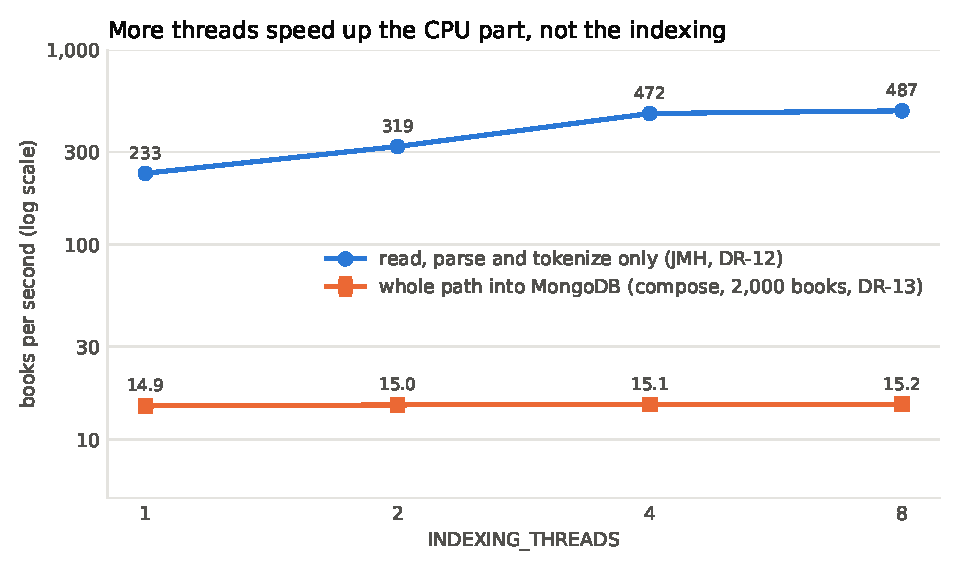
\includegraphics[width=0.49\linewidth]{figures/index_threads.pdf}\hfill
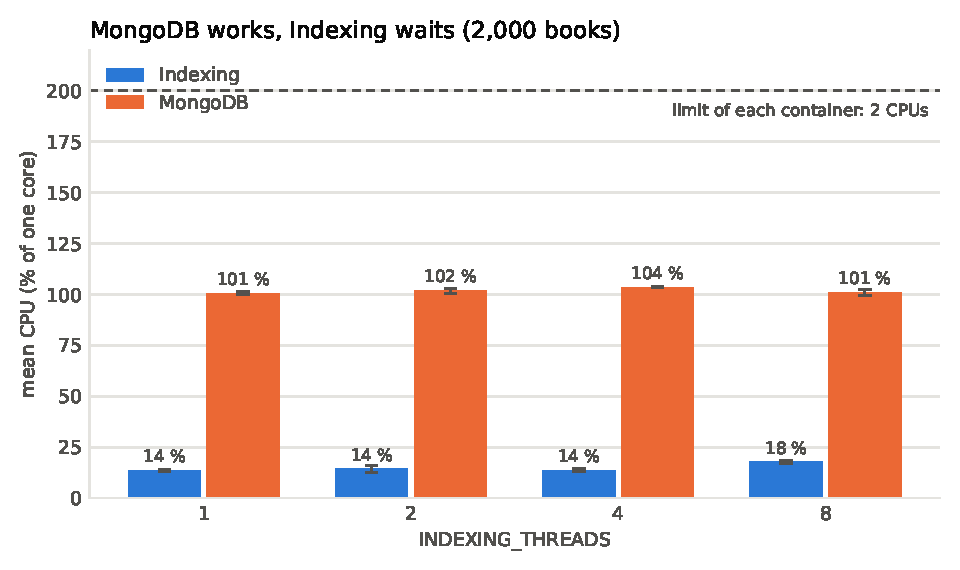
\includegraphics[width=0.49\linewidth]{figures/index_threads_cpu.pdf}
\caption{Left: books per second against the parser threads, for the CPU part alone (JMH) and for the whole path into
MongoDB. Right: mean CPU of Indexing and MongoDB in those runs.}
\label{fig:index-threads}
\end{figure}

\textbf{Scale.} 4 threads, 1 replica; 30,000 books ran once because one run takes more than 4~hours:

\begin{table}[H]
\centering\small
\begin{tabular}{@{}rrrrrrr@{}}
\toprule
\textbf{Books} & \textbf{Runs} & \textbf{Books/s} & \textbf{Duration} & \textbf{Terms} & \textbf{Index on disk} &
  \textbf{Longest list} \\
\midrule
200 & 3 & 24.90 $\pm$ 0.02 & 11 s & 58,244 & 5.8 MB & 200 ids \\
10,000 & 3 & 5.54 $\pm$ 0.01 & 30 min & 394,502 & 465 MB & 9,965 ids, 99 KB \\
30,000 & 1 & 2.00 & 4 h 10 min & 651,565 & 1.11 GB & 29,898 ids, 318 KB \\
\bottomrule
\end{tabular}
\caption{Indexing against the number of books. Peak memory: Indexing 404 to 518~MiB, MongoDB 461 to 802~MiB of its
1~GB, Hazelcast 326 to 390~MiB.}
\label{tab:index-scale}
\end{table}

\begin{figure}[H]
\centering
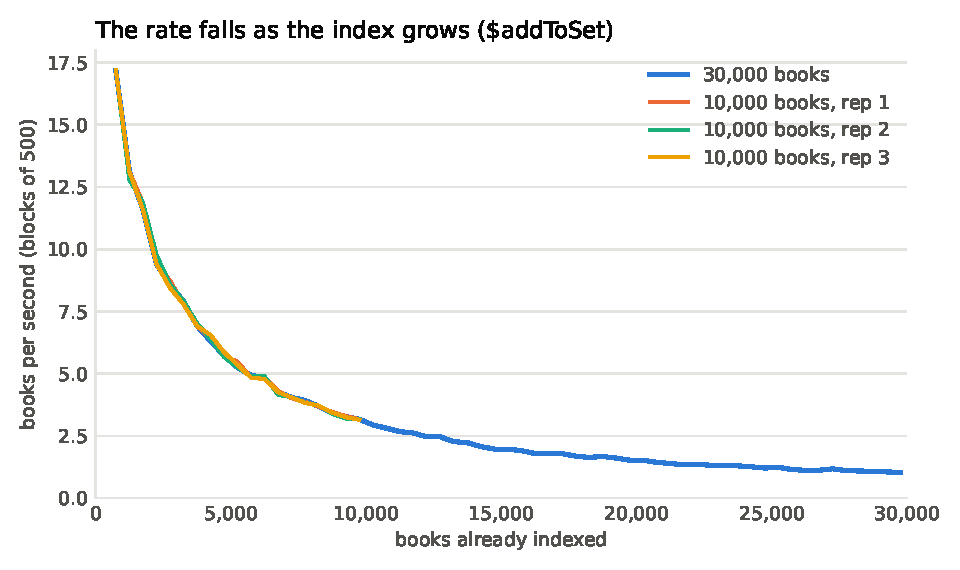
\includegraphics[width=0.75\linewidth]{figures/index_rate.pdf}
\caption{Books per second against the books already in the index, in blocks of 500 books (5 batches). The three runs
of 10,000 books and the run of 30,000 lie on one curve.}
\label{fig:index-rate}
\end{figure}

\textbf{Probe of the posting lists.} To isolate the cost of one update, the driver adds 100 ids to a single posting
list of a given length, 20 times, with \code{\$addToSet} and with \code{\$push}:

\begin{figure}[H]
\centering
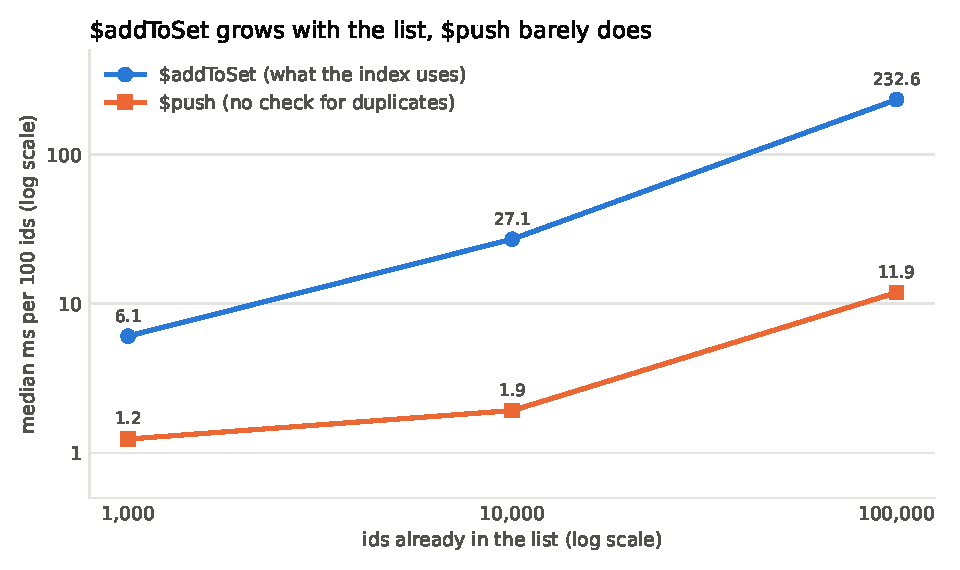
\includegraphics[width=0.49\linewidth]{figures/index_probe.pdf}\hfill
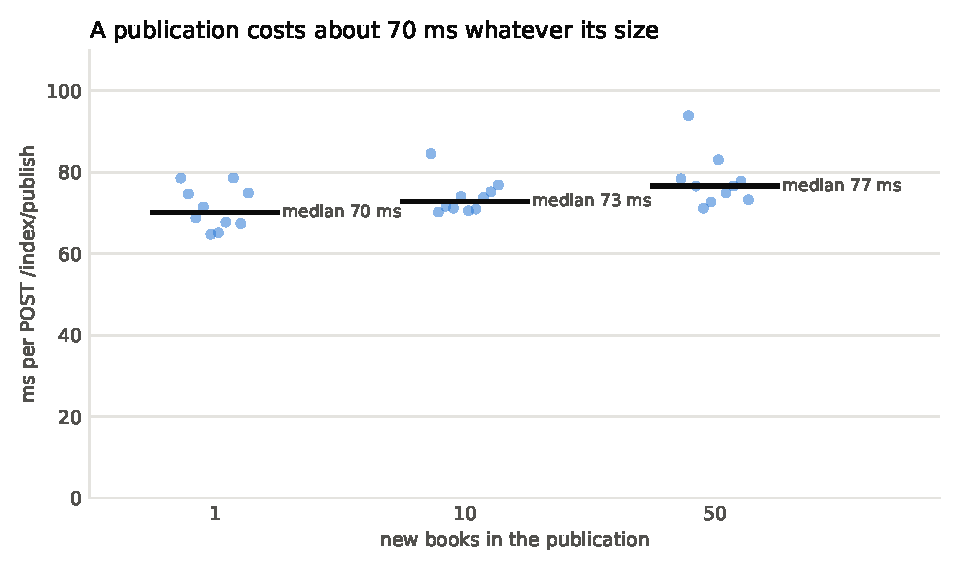
\includegraphics[width=0.49\linewidth]{figures/index_publish.pdf}
\caption{Left: median time to add 100 ids to one posting list. Right: each \code{POST /index/publish} of 1, 10 and 50
new books on an index of 10,000 books, 10 times each, and the median.}
\label{fig:index-probe-publish}
\end{figure}

\textbf{Publication.} \code{POST /index/publish} on an index of 10,000 books takes a median of 70, 73 and 77~ms for 1, 10
and 50 new books (Figure~\ref{fig:index-probe-publish}). The first publication, with all 10,000 books, took 459~ms.

\subsection{Analysis}

\begin{itemize}
  \item \textbf{Indexing is limited by MongoDB, not by its own CPU.} From 1 to 8 threads the rate improves by 2~\%,
        within the noise, while the CPU part alone doubles. Indexing uses less than a fifth of one core. MongoDB uses
        about one core of its two for the whole run, because a single writer sends one bulk write at a time: the work
        of MongoDB is one serial stream.
  \item \textbf{The rate falls as the index grows, and \code{\$addToSet} explains it.} At 10,000 books a batch of 100
        takes about 33~s, at 30,000 about 90~s. The probe shows why: \code{\$addToSet} compares each new id with the
        whole list, so its cost grows linearly with the list, 14 times that of \code{\$push} at 10,000 ids and 20 times
        at 100,000. The frequent terms hold almost one id per book, so every batch pays for the size of the index.
        The two scales agree where they overlap: books 9,000 to 12,000 of the 30,000 run went at 2.9 books/s, and the
        last tenth of the 10,000 runs at 3.2.
  \item \textbf{Publishing is cheap and its cost is fixed.} From 1 to 50 new books the median grows by 7~ms: the round
        trips of its steps dominate, not the books. The Control can therefore publish often, every 30~s or every 100
        books, without loading MongoDB.
  \item \textbf{Saturation point.} On this host and these limits, indexing does not saturate a resource of its own: it
        is bound by the time MongoDB takes per update, which grows with the index. Adding threads or replicas to
        Indexing changes nothing; changing the write (Section~\ref{sec:decisions-storage}) or giving MongoDB more cache
        and CPU would.
\end{itemize}

\textbf{Limits of these measures.}
\begin{itemize}
  \item Everything runs on one machine: the driver, \code{docker stats} and the services share its CPUs.
  \item The WiredTiger cache (0.25~GB) is smaller than the index from 10,000 books on. The probe isolates
        \code{\$addToSet} on one document, but in the full runs part of the slowdown may also come from the cache.
  \item MongoDB is not restarted between runs, only its database is deleted, so its peak memory grows along the run
        whatever the level.
  \item With 200 books only 1 or 2 samples of the monitor fall inside the run, so its CPU figures are not meaningful.
  \item 100,000 books were not measured: even at the rate of the last books of the 30,000 run, about one book per
        second and still falling, the 70,000 more books would take over 19~hours.
  \item Indexing replicas were not measured for throughput: by design only one writes. Their failover was measured
        (Section~\ref{sec:indexing}).
\end{itemize}

\section{Benchmarks and results: consolidation}
\label{sec:consolidation}

This part puts the measures of the three services side by side: one host, the configurations measured, and where each
part of the system saturates.

\subsection{The host}

Every valid measure ran on one machine, recorded by the \code{host.txt} of each run:

\begin{table}[H]
\centering\small
\begin{tabularx}{\linewidth}{@{}L{3.4cm}X@{}}
\toprule
CPU & Intel Core i7-9750H, 2.60~GHz: 6 cores, 12 logical CPUs \\
Memory and storage & 16~GB; NVMe SSD \\
Operating system & Ubuntu 24.04.5, Linux 7.0 \\
Docker & 28.3.3, sees the 12 CPUs and 16~GB \\
JVM & OpenJDK 21.0.12 for JMH and the drivers; the images run Java 17 \\
Power & Plugged in, balanced energy profile \\
\bottomrule
\end{tabularx}
\caption{Reference machine of all the benchmarks.}
\label{tab:host}
\end{table}

The deployment limits each container (\code{.env}): MongoDB 2 CPUs and 1~GB with a 0.25~GB cache; Indexing 2 CPUs and
1~GB; Search 2 CPUs per replica; Ingestion 1 CPU and 512~MB; each Hazelcast member 1 CPU and 768~MB; the Control and
nginx 0.5 CPUs. The load experiments of Search give nginx 2 CPUs, so that it does not hide the rest, and measure its
0.5 CPUs apart. The limits together exceed the 12 CPUs of the host only in the Search experiments with 4 replicas
(14 CPUs), where the replicas compete for the same cores.

\subsection{What was measured}

\begin{table}[H]
\centering\small
\begin{tabularx}{\linewidth}{@{}L{3.1cm}L{2.2cm}L{2.2cm}X@{}}
\toprule
\textbf{Experiment} & \textbf{Scope} & \textbf{Replicas} & \textbf{Threads and clients} \\
\midrule
Ingestion JMH & component, host & -- & 1, 2, 4, 8 workers \\
Indexing JMH & component, host & -- & 1, 2, 4, 8 parser threads \\
Search JMH & component, host & -- & 1, 2, 4, 8 threads \\
Indexing, threads & Indexing + MongoDB + Hazelcast, Docker & 1 Indexing & 1, 2, 4, 8 parser threads; 2,000 books \\
Indexing, scale & same & 1 Indexing & 4 threads; 200, 10,000, 30,000 books \\
Indexing, publication & same & 1 Indexing & 1, 10, 50 new books on 10,000 \\
Search, load & Search + MongoDB + nginx, Docker & 1, 2, 4 Search & 1 to 256 closed-loop clients; 250 Jetty threads
  (also 16 and 64); pool of 50 (also 10 and 100); nginx with 2 CPUs (also 0.5); index of 15, 197 and 10,000 books \\
Search with the pipeline & complete pipeline, Docker & 1 of each & 32 and 128 clients on 2,000 books while the
  pipeline processes new ones \\
\bottomrule
\end{tabularx}
\caption{The experiments, each labelled with what it measures. Every configuration was repeated 3 times, except the
30,000 books of Indexing (once). Client concurrency, replicas and threads are kept apart.}
\label{tab:experiments}
\end{table}

\subsection{Bottlenecks and scaling trends}

\begin{table}[H]
\centering\small
\begin{tabularx}{\linewidth}{@{}L{1.9cm}L{4.4cm}X@{}}
\toprule
\textbf{Service} & \textbf{Measured rate} & \textbf{What limits it} \\
\midrule
Ingestion & 473 $\mu$s per book with 1 worker, 155 with 8 (local source, JMH) &
  The coordination: claim and complete cost 1.6~ms per book with 1 thread and 0.36 with 8, more than the ingestion
  itself. With Project Gutenberg the download is far longer than both. \\
Indexing & 15 books/s on 2,000 books; 5.5 on 10,000; 2.0 on 30,000 &
  MongoDB: the cost of \code{\$addToSet} grows with each posting list, and one writer sends one stream of writes.
  Threads and replicas of Indexing do not change it (Section~\ref{sec:benchmarks-indexing}). \\
Search & About 7,500 req/s on 15 books whatever the replicas; on 10,000 books 1,036 req/s with 1 replica and
  2,612 with 4 &
  On a small index MongoDB is the limit: it reaches its 2 CPUs while the replicas of Search have CPU to spare. On
  10,000 books each query matches most of the index, the CPU of Search is the limit, and replicas help: 4 give 2.5
  times the peak of one, less than 4 because the host runs out of CPU (Section~\ref{sec:benchmarks}). \\
The whole system & with the pipeline running, Search 2,600 req/s and Indexing 0.91 books/s at the same time &
  MongoDB is shared: the writes of Indexing take it from 80 to 191~\% of its 2 CPUs. Indexing drops from 2.42 to
  0.91 books/s while Search is under load, and the p95 of Search with 128 clients rises from 109 to 160~ms. \\
\bottomrule
\end{tabularx}
\caption{Where each part of the system saturates on the reference machine.}
\label{tab:bottlenecks}
\end{table}

\textbf{Threads and replicas.} Threads help where the work is CPU inside one process: the workers of Ingestion and the
parsers of Indexing in JMH, and the replicas of Search when queries are long. They do not help where the limit is a shared
resource: the queue of Hazelcast for Ingestion with small books, MongoDB for Indexing, and MongoDB again for Search
on a small index. Indexing replicas are
standbys by design, so their effect is failover, not throughput.

\textbf{What was not measured.} The full pipeline with several Ingestion replicas and Project Gutenberg as the source
(the measures use the local source, so that the network does not dominate); 100,000 books, because indexing them at the
measured rate would take most of a day; and two machines, which is Stage~3.


\end{document}
